%----------------------------------------------------------------
\chapter{Getting information From Tao}
\label{c:get.info}

To use \tao with this chapter, please starup \tao as explained in \sref{s:obtaining} in 
the \vn{introduction_to_tao} directory that you have copied to your local area.

%----------------------------------------------------------------
\section{The Plotting Window}
\index{plotting}

When \tao first starts up, \tao will create a new window for
displaying plots. This window will be called the \vn{plot}
window. Commands to \tao can be typed in from the original window from
which \tao was invoked. This will be called the \vn{command} window.

Figure~\ref{f:plot.begin} shows what you will see in the plot window. In the top two plots you see
the \vn{x} and \vn{y} model lattice orbit data. The horizontal axis is the \cesr BPM index. The
horizontal pretzel and L03 vertical bump in CESR can be clearly seen. The slight vertical
displacement due to the solenoid compensation can also be seen around the IP. The orbit data is for
a closed orbit electron (this being a storage ring). The bottom two plots show the relative particle
phase, that is, the difference between the model and design phases (as documented in the plot title
as [model - design]). 

As a first step, let us command \tao to display some plotting
information using the command:
\begin{example}
  show plot       ! \sref{s:show}
\end{example}
The information will be displayed in the command window. The first
section of the \vn{show plot} output shows information on font sizes:
\begin{example}
  plot_page parameters:
  %size                         =   400  500
  %n_curve_pts                  =   401
  %text_height                  = 12.000
  %main_title_text_scale        = 1.300
  %graph_title_text_scale       = 1.100
  %axis_number_text_scale       = 0.900
  %axis_label_text_scale        = 1.000
  %key_table_text_scale         = 0.900
  %legend_text_scale            = 0.700
  %floor_plan_shape_scale       = 1.000
  %lat_layout_shape_scale       = 1.000
  %delete_overlapping_plots     = T
\end{example}
See section~\sref{s:init.plot} for more details. 

The second section of the \vn{show plot} output lists the plot \vn{templates} (\sref{c:plotting} and
\sref{s:template}) that \tao knows about:
\begin{example}
 Templates:
   Plot               
   ------------------ 
   orbit              
   phase              
   beta               
   eta                
   cbar               
   quad_k1
   floor              
\end{example}
The template plots come from two sources. First templates are defined, in this example, in the
\vn{tao_plot.init} file. Second, \tao defines a set of default templates.

%---------------------------

\begin{figure}[tb]
  \centering
  \begin{subfigure}[b]{0.48\textwidth}
    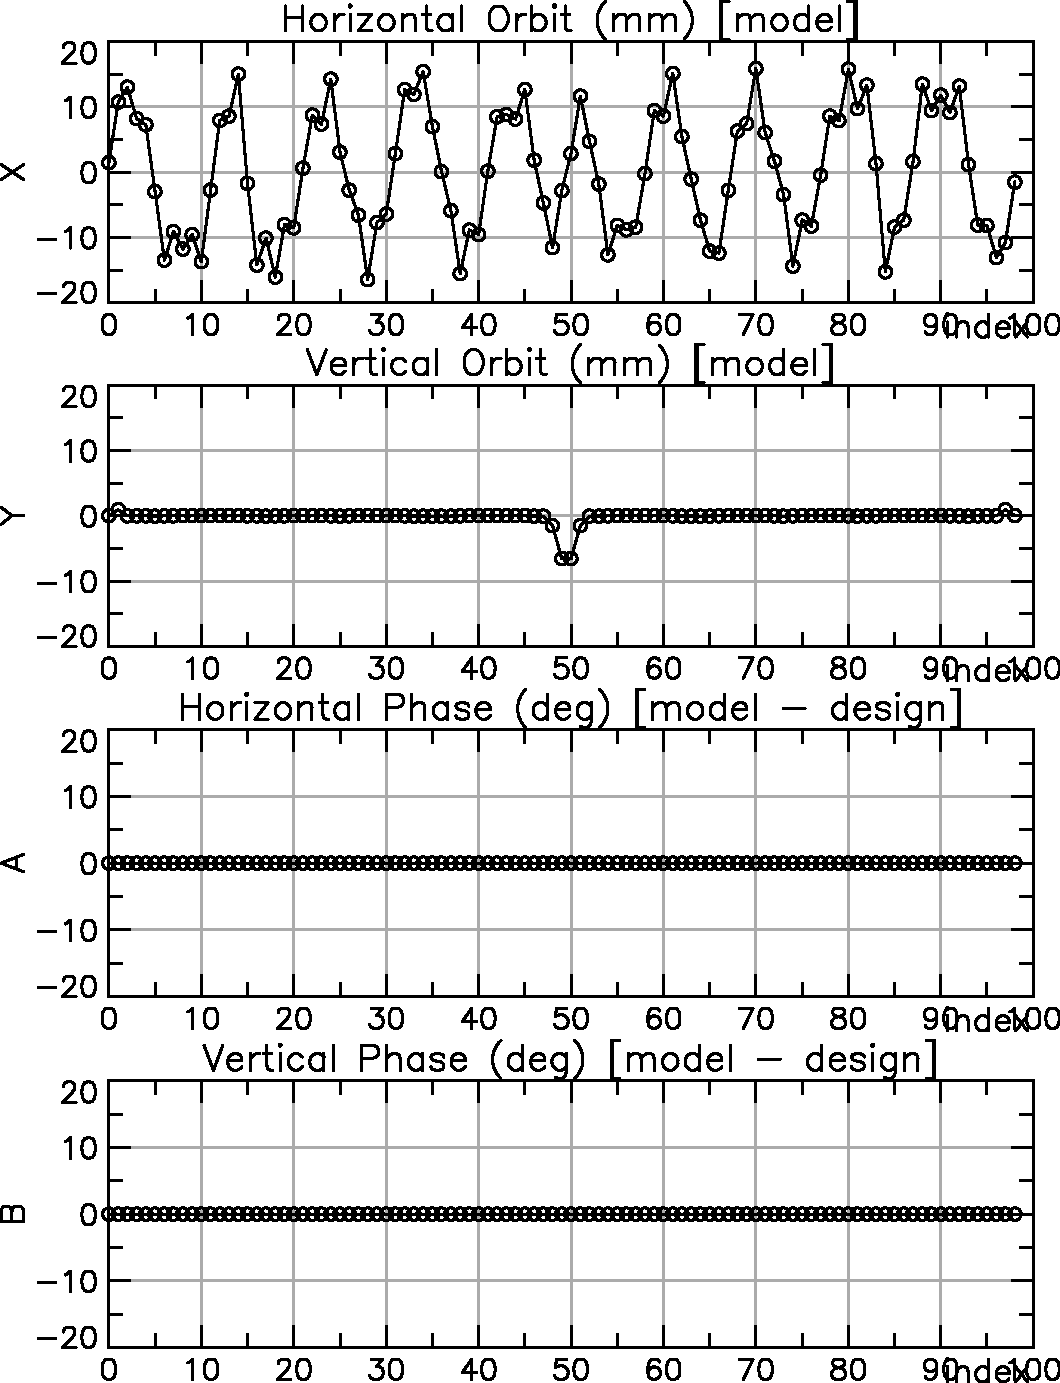
\includegraphics[width=3in]{plot-page1.pdf}
    \caption{The plot window at startup}
    \label{f:plot.begin}
  \end{subfigure}
  \begin{subfigure}[b]{0.48\textwidth}
    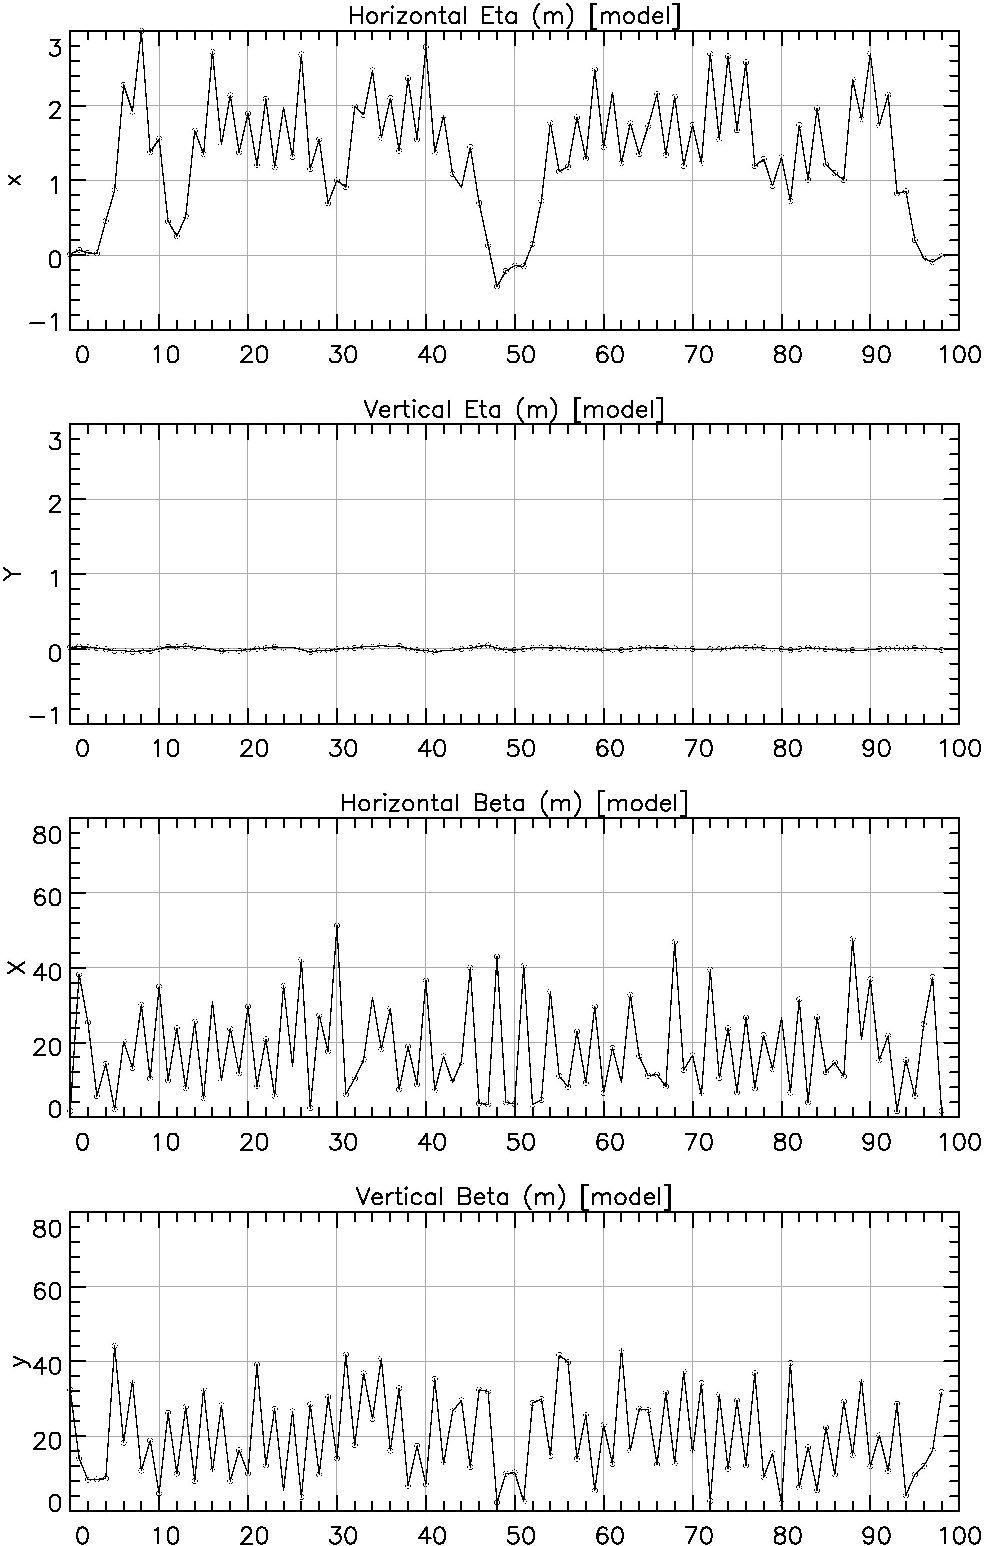
\includegraphics[width=3in]{plot-eta-beta.pdf}
    \caption{Plotting dispersion and beta function}
    \label{f:plot.eta.beta}
  \end{subfigure}
  \caption{Example plots.}
\end{figure}

%---------------------------

The next block of information in the \vn{show plot} command are the regions in which
template plots have been placed:
\begin{example}
  Plot Region         <-->  Plot                 x1    x2    y1    y2
  -----------               -----------------------------------------
  top                 <-->  orbit               0.00  1.00  0.48  0.95
  bottom              <-->  phase               0.00  1.00  0.00  0.48
  layout              <-->                      0.00  1.00  0.00  0.15
  r11                 <-->                      0.00  1.00  0.15  1.00
  r12                 <-->                      0.00  1.00  0.58  1.00
  ... etc...
\end{example}
Plot regions (\vn{top}, \vn{bottom}, and \vn{layout}) are defined, in this example, in the
\vn{tao_plot.init} file. Additional default plot regions, all beginning with the letter \vn{r}, are
defined by \tao. Here, the \vn{top} plot contains an \vn{orbit} plot and the \vn{bottom} region
contains a betatron \vn{phase} plot.

To see information on, say, the orbit plot, use the command
\begin{example}
  show plot orbit
\end{example}
This shows:
\begin{example}
  Region:  orbit
  Plot:  orbit
  x_axis_type          = index
  x%label              =
  x%max                =   1.00000000E+02
  x%min                =   0.00000000E+00
  x%major_div          =       10
  x%major_div_nominal  =       10
  x%places             =       -1
  x%draw_label         = T
  x%draw_numbers       = T
  autoscale_x          = F
  autoscale_y          = F
  autoscale_gang_x     = T
  autoscale_gang_y     = T
  Graphs:
     x
     y
\end{example}
This command shows that the \vn{orbit} plot has two associate graphs (\sref{c:plotting}) called
\vn{x} and \vn{y}.  To see information on, say, the \vn{x} graph use the command 
\begin{example}
  show graph orbit.x    ! \sref{s:show.graph}
\end{example}
Similarly, the \vn{show curve} (\sref{s:show.curve}) command can be used to display
information about the curves within each graph.

Also see the \vn{show graph} and \vn{show curve} commands.
Section~\sref{s:init.plot} has information on the plot parameters.

\index{commands!plot}
Let's view the absolute model phase. Use the command:
\begin{example}
  set plot bottom component = model
\end{example}
This will change the data plotted in the bottom two graphs to just the
model.  The plotted curves are now way off scale. Let \tao automatically set
the scale by typing:
\index{commands!scale}
\begin{example}
  scale bottom
\end{example}
As expected, the phase increases approximately linearly as the particle travels through the
ring. Zero phase is about halfway through the ring. This is due to the fact that the absolute phase
is arbitrary so \tao sets the average phase to zero when plotting phase data. To set the plot back to
relative phase type:
\begin{example}
  set plot bottom component = model - design
\end{example}

Let's now look at the beta function by typing
\index{commands!place}
\begin{example}
  place bottom beta
\end{example}
Again, we need to rescale the plots by typing
\index{commands!scale}
\begin{example}
  scale bottom
\end{example}
We see the periodic FODO beta function where large horizontal beta
corresponds to small vertical beta and vice versa.

Likewise, we can look at the dispersion in the top two graphs by
typing
\index{commands!scale}
\begin{example}
  place top eta
  scale top
\end{example}
The plot window should now look like Figure~\ref{f:plot.eta.beta}.

Now let's look at the coupling (C-matrix) by typing
\begin{example}
  place bottom cbar
  scale bottom
\end{example}
We see that there is strong coupling within the CLEO solenoid (at the left and right edges of the
plot) and virtually no coupling anywhere else. To zoom in the scale so that we can see the residual
coupling outside the interaction region type
\begin{example}
  scale bottom -0.01 0.01
\end{example}
The \vn{**Curve Off Scale**} displayed in red on the bottom plots tells us that there are data
points outside the plotted region.  We now see that there is a small amount of coupling throught the
lattice.

The x-axis is currently the BPM index number. It is sometimes
convenient to plot the data versus longitudinal position. This is done
by typing
\index{commands!x-axis}
\begin{example}
  x-axis * s
\end{example}

%------------------------

\begin{figure}
  \centering
  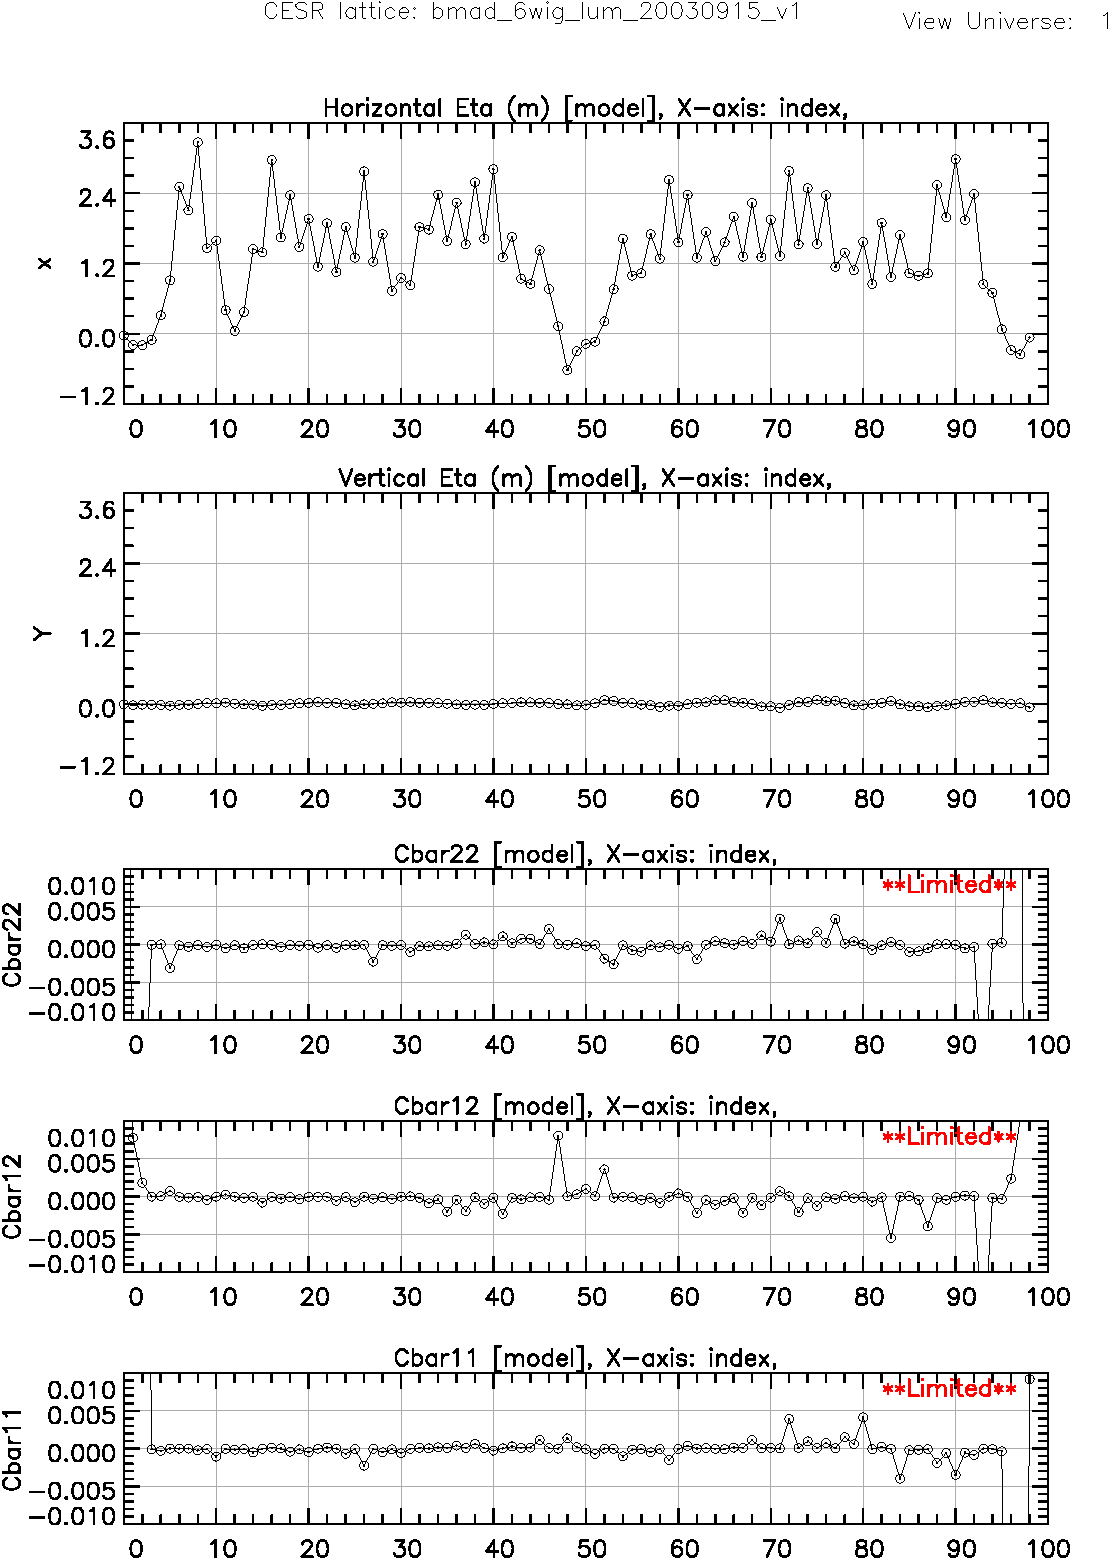
\includegraphics[width=3in]{plot-coupling-no-IR.pdf}
  \caption{Cbar and quarupole K1 plots.}
  \label{f:plot.coupling.no.IR}
\end{figure}

%------------------------

The \cmd{all} will apply the change to all plot areas (both top and
bottom). In any of the above commands \cmd{top} or \cmd{bottom} could
have been replaced with \cmd{all}.

Variables can also be plotted provided the proper plot template has
been set up in the plot initialization file (See
Section~\sref{s:init.plot} for details on initializing plotting). Type
the following to view the quadrupole k1 values:
\begin{example}
  place top quad_k1
\end{example}
Your plot window should now look like Figure~\ref{f:plot.coupling.no.IR}.
\index{commands!plot}
\index{commands!place}

%----------------------------------------------------------------
\section{The Show Command}

Anything in the super-universe can be displayed using the \cmd{show}
command (\sref{s:show}). To get a list of the data elements currently
defined in \tao type
\index{commands!show}
\begin{example}
  show data
\end{example}
the output should look like:
\begin{example}
  Name                                   Using for Optimization

  orbit.x[0:99]
  orbit.y[0:99]

  phase.a[0:99]
  phase.b[0:99]

  eta.x[0:99]
  eta.y[0:99]

  beta.a[0:99]
  beta.b[0:99]

  cbar.11[0:99]
  cbar.12[0:99]
  cbar.21[0:99]
  cbar.22[0:99]

  k.11b[0:99]
  k.12a[0:99]
  k.12b[0:99]
  k.22a[0:99]
\end{example}
There are six \vn{d2} data types (\sref{s:data.org}) defined in the
initialization file: \vn{orbit}, \vn{phase}, etc.  The \vn{beta} data is further
subdivided into two \vn{d1} data arrays labeled \vn{beta.a} and \vn{beta.b}.
Each of these arrays has 100 data points indexed from 0 to 99.

The \vn{``Using for Optimization''} column is blank indicating that no data
would be used in an optimization (\sref{c:opti}).

To see the data values for the horizontal beta function for \cesr BPMs
1 through 50 type
\begin{example}
  show data beta.a[1:50]
\end{example}
Since we haven't changed any elements in the lattice yet the model
values equal the design values. Also note that \vn{beta.a} is actually
the a-mode betatron function. In regions with little or no coupling,
the a-mode is almost completely in the horizontal plane.

A significant point: The convention in \bmad is to label the twiss
parameters as \vn{x} and \vn{y} but they are actually the \vn{a} and
\vn{b} normal modes. So in regions of strong coupling \vn{beta.a} does
not correspond to \vn{orbit.x} which is always in the true horizontal
lab frame.  However, if you wish, you can re-label your twiss data
planes as \vn{a} and \vn{b}.  Section~\ref{c:init} shows you how to do
this. Keep in mind that lattice twiss parameters are defined
\textit{only for uncoupled betatron motion} so this is all that is
provided as data types for single particle tracking.  However, true
lab-frame \vn{x} and \vn{y} twiss parameters can be defined for a
distribution of particles so for beam
tracking true lab-frame \vn{x} and \vn{y} twiss parameters can be
calculated and are provided as data types for those tracking
types. See the \bmad manual for how to convert from normal mode
coordinates to lab-frame coordinates.

This tutorial uses single particle tracking and the twiss parameters
are found about the orbit of the tracked particle. There is another
tracking type called particle beam tracking. This
tracking type will not be explored in this tutorial.

You can also view variables by typing
\begin{example}
  show var
\end{example}
To view the quadrupole k1 values for \cesr quadrupoles 5 and 20
through 30 type
\begin{example}
  sho var quad\_k1[5,20:30]
\end{example}
Again, since we haven't changed any quadrupoles the model values are
all at their design values.

You can also see the details of a particular lattice element. To view
the details for quadrupole Q05W type
\begin{example}
  sho ele Q05W
\end{example}

\vn{show var} and \vn{show ele} show two completely different types of
structures in \tao. Elements are the actual lattice elements as known
to \bmad.  Variables are native \tao structures that act kind of like
\bmad \textit{overlays} and only indirectly control the lattice
elements.

A list of lattice elements between two elements can be shown by typing 
\begin{example}
  sho lattice 0:20
\end{example}
This will show a list of all the lattice elements between and
including elements 0 and 20. Twiss parameters and orbit information, at
the exit end of each element, is also shown.

Anything printed to the display using the \vn{show} command can also
be printed to a file by typing
\begin{example}
  show -write <file_name> <what_to_show>
\end{example}
\index{commands!show}

A list of all intrinsic \vn{tao} commands can be found by typing
\index{commands!help}
\begin{example}
  help
\end{example}
This will not list any custom commands. Detailed help on any
individual command can be found with
\begin{example}
  help <command\_name>
\end{example}
where \vn{<command_name>} is the command you want help with.
